\chapter{Primaria}
Bien empezare escribiendo que al igual que en le kinder asisti a dos esculas primarias las culas fueron las siguientes:
\begin{itemize}
	\item Primaria
		\begin{itemize}
			\item	Ignacio Manuel Altamirano
			\item	Telposcalli
		\end{itemize}
\end{itemize}

En la escuala Ignacio Manuel Altamirano me parecio mucho mejor que las Telposcalli devido a que primero ingrese a la Escula Primaria Iganacio Manuel Altamirano estube hay 5 de los 6 años que tenemos que estar en la primaria
pero despues a mi padre se le ocurrio la "marabillosa idea" de cambiarme ala Telposcalli el ultimo año y pues como era nuevo no conosia a muchos pero al final todos me terminaron conociendo porque igual que en el kinder tenia una tia en dicha escuela, pero donde mas me diverti y aprendi fue en la Escuela Igancio Manuel Altamirano.

\begin{figure}[H]
\centering
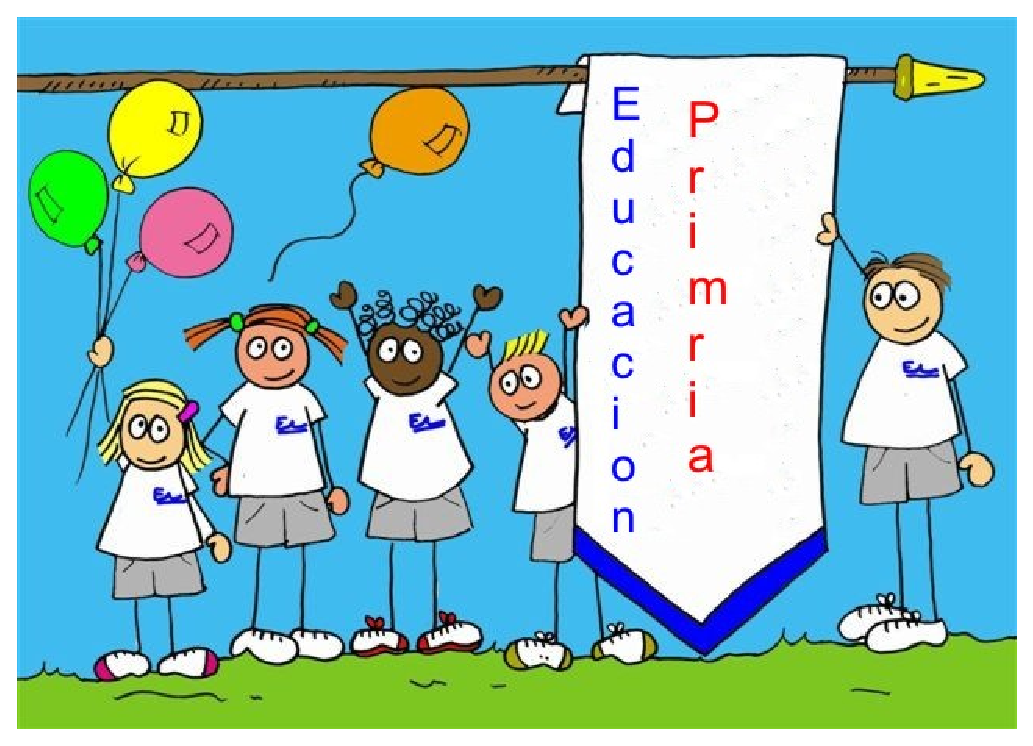
\includegraphics[width=.5\textwidth]{treeChapter/primaria.eps}
\caption{la formacion Primaria}
\label{Primaria}	
\end{figure}
